%%%% Paramétrage du TD %%%%
\def\xxactivite{TD 01 \ifprof-- Corrigé \else \fi }
\def\xxauteur{\textsl{Xavier Pessoles}}
%\fancyfoot[C]{\rule{12cm}{.5pt}}
%\renewcommand{\footrulewidth}{0.2pt}
%\fancyfoot[C]{\footnotesize{\bfseries \thepage}}
%\fancyfoot[L]{ 
%\begin{minipage}[c]{.4\linewidth}
%\noindent\footnotesize{{\xxauteur}}
%\end{minipage}}


\def\xxnumchapitre{Chapitre 2 \vspace{.2cm}}
\def\xxchapitre{\hspace{.12cm} Rapidité des systèmes}

\def\xxcompetences{%
\textsl{%
\textbf{Savoirs et compétences :}\\
\vspace{-.4cm}
%\begin{itemize}[label=\ding{112},font=\color{ocre}] 
%\item \textit{Mod3.C2 : } pôles dominants et réduction de l’ordre du modèle : principe, justification
%\item \textit{Res2.C4 : } stabilité des SLCI : définition entrée bornée -- sortie bornée (EB -- SB)	
%\item \textit{Res2.C5 : } stabilité des SLCI : équation caractéristique	
%\item \textit{Res2.C6 : } stabilité des SLCI : position des pôles dans le plan complexe
%\item \textit{Res2.C7 : } stabilité des SLCI : marges de stabilité (de gain et de phase)
%\end{itemize}
}}


\def\xxfigures{
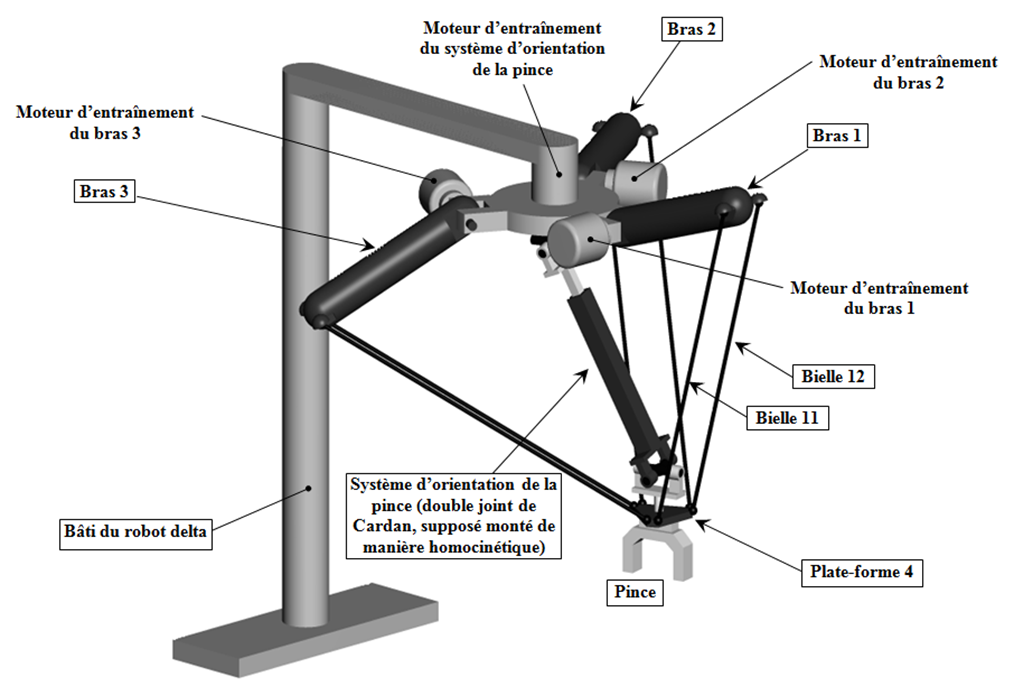
\includegraphics[width=.4\linewidth]{fig_01}
}%figues de la page de garde

\def\xxtitreexo{Robot de consolidation de parois rocheuses Roboclimber}
\def\xxsourceexo{\hspace{.2cm} \footnotesize{Mines Ponts PSI 2011 -- Éditions Vuibert}}

\iflivret
\pagestyle{empty}


%%%%%%%% PAGE DE GARDE COURS
\ifcours
\begin{tikzpicture}[remember picture,overlay]
\node at (current page.north west)
{\begin{tikzpicture}[remember picture,overlay]
\node[anchor=north west,inner sep=0pt] at (0,0) {\includegraphics[width=\paperwidth]{\thechapterimage}};
\draw[anchor=west] (-2cm,-8cm) node [line width=2pt,rounded corners=15pt,draw=ocre,fill=white,fill opacity=0.6,inner sep=40pt]{\strut\makebox[22cm]{}};
\draw[anchor=west] (1cm,-8cm) node {\huge\sffamily\bfseries\color{black} %
\begin{minipage}{1cm}
\rotatebox{90}{\LARGE\sffamily\textsc{\color{ocre}\textbf{\xxnumpartie}}}
\end{minipage} \hfill
\begin{minipage}[c]{14cm}
\begin{titrepartie}
\begin{flushright}
\renewcommand{\baselinestretch}{1.1} 
\Large\sffamily\textsc{\textbf{\xxpartie}}
\renewcommand{\baselinestretch}{1} 
\end{flushright}
\end{titrepartie}
\end{minipage} \hfill
\begin{minipage}[c]{3.5cm}
{\large\sffamily\textsc{\textbf{\color{ocre} \discipline}}}
\end{minipage} 
 };
\end{tikzpicture}};
\end{tikzpicture}


\begin{tikzpicture}[overlay]
\node[shape=rectangle, 
      rounded corners = .25 cm,
	  draw= ocre,
	  line width=2pt, 
	  fill = ocre!10,
	  minimum width  = 2.5cm,
	  minimum height = 3cm,] at (18cm,0) {};
\node at (17.7cm,0) {\rotatebox{90}{\textbf{\Large\color{ocre}{\classe}}}};
%{};
\end{tikzpicture}

\vspace{3.5cm}

\begin{tikzpicture}[remember picture,overlay]
\draw[anchor=west] (-2cm,-6cm) node {\huge\sffamily\bfseries\color{black} %
\begin{minipage}{2cm}
\begin{center}
\LARGE\sffamily\textsc{\color{ocre}\textbf{\xxactivite}}
\end{center}
\end{minipage} \hfill
\begin{minipage}[c]{15cm}
\begin{titrechapitre}
\renewcommand{\baselinestretch}{1.1} 
\Large\sffamily\textsc{\textbf{\xxnumchapitre}}

\Large\sffamily\textsc{\textbf{\xxchapitre}}
\vspace{.5cm}

\renewcommand{\baselinestretch}{1} 
\normalsize\normalfont
\xxcompetences
\end{titrechapitre}
\end{minipage}  };
\end{tikzpicture}
\vfill

\begin{flushright}
\begin{minipage}[c]{.3\linewidth}
\begin{center}
\xxfigures
\end{center}
\end{minipage}\hfill
\begin{minipage}[c]{.6\linewidth}
\startcontents
\printcontents{}{1}{}
\end{minipage}
\end{flushright}

\begin{tikzpicture}[remember picture,overlay]
\draw[anchor=west] (4.5cm,-.7cm) node {
\begin{minipage}[c]{.2\linewidth}
\begin{flushright}

\includegraphics[width=2cm]{png/logoCC}
\end{flushright}
\end{minipage}
\begin{minipage}[c]{.2\linewidth}
\textsl{\xxauteur} \\
\textsl{\classe}
\end{minipage}
 };
\end{tikzpicture}
\newpage
\pagestyle{fancy}

\newpage
\pagestyle{fancy}

\else
\fi


%%%%%%%% PAGE DE GARDE TD
\iftd
%\begin{tikzpicture}[remember picture,overlay]
%\node at (current page.north west)
%{\begin{tikzpicture}[remember picture,overlay]
%\draw[anchor=west] (-2cm,-3.25cm) node [line width=2pt,rounded corners=15pt,draw=ocre,fill=white,fill opacity=0.6,inner sep=40pt]{\strut\makebox[22cm]{}};
%\draw[anchor=west] (1cm,-3.25cm) node {\huge\sffamily\bfseries\color{black} %
%\begin{minipage}{1cm}
%\rotatebox{90}{\LARGE\sffamily\textsc{\color{ocre}\textbf{\xxnumpartie}}}
%\end{minipage} \hfill
%\begin{minipage}[c]{13.5cm}
%\begin{titrepartie}
%\begin{flushright}
%\renewcommand{\baselinestretch}{1.1} 
%\Large\sffamily\textsc{\textbf{\xxpartie}}
%\renewcommand{\baselinestretch}{1} 
%\end{flushright}
%\end{titrepartie}
%\end{minipage} \hfill
%\begin{minipage}[c]{3.5cm}
%{\large\sffamily\textsc{\textbf{\color{ocre} \discipline}}}
%\end{minipage} 
% };
%\end{tikzpicture}};
%\end{tikzpicture}

%%%%%%%%%% PAGE DE GARDE TD %%%%%%%%%%%%%%%
%\begin{tikzpicture}[overlay]
%\node[shape=rectangle, 
%      rounded corners = .25 cm,
%	  draw= ocre,
%	  line width=2pt, 
%	  fill = ocre!10,
%	  minimum width  = 2.5cm,
%	  minimum height = 2.5cm,] at (18.5cm,0) {};
%\node at (17.7cm,0) {\rotatebox{90}{\textbf{\Large\color{ocre}{\classe}}}};
%%{};
%\end{tikzpicture}

% PARTIE ET CHAPITRE
%\begin{tikzpicture}[remember picture,overlay]
%\draw[anchor=west] (-1cm,-2.1cm) node {\large\sffamily\bfseries\color{black} %
%\begin{minipage}[c]{15cm}
%\begin{flushleft}
%\xxnumchapitre \\
%\xxchapitre
%\end{flushleft}
%\end{minipage}  };
%\end{tikzpicture}

% Bandeau titre exo
\begin{tikzpicture}[remember picture,overlay]
\draw[anchor=west] (-2cm,-4cm) node {\huge\sffamily\bfseries\color{black} %
\begin{minipage}{5cm}
\begin{center}
\LARGE\sffamily\color{ocre}\textbf{\textsc{\xxactivite}}

\begin{center}
\xxfigures
\end{center}

\end{center}
\end{minipage} \hfill
\begin{minipage}[c]{12cm}
\begin{titrechapitre}
\renewcommand{\baselinestretch}{1.1} 
\large\sffamily\textbf{\textsc{\xxtitreexo}}

\small\sffamily{\textbf{\textit{\color{black!70}\xxsourceexo}}}
\vspace{.5cm}

\renewcommand{\baselinestretch}{1} 
\normalsize\normalfont
\xxcompetences
\end{titrechapitre}
\end{minipage}  };
\end{tikzpicture}

\else
\fi


%%%%%%%% PAGE DE GARDE FICHE
\iffiche
\begin{tikzpicture}[remember picture,overlay]
\node at (current page.north west)
{\begin{tikzpicture}[remember picture,overlay]
\draw[anchor=west] (-2cm,-3.25cm) node [line width=2pt,rounded corners=15pt,draw=ocre,fill=white,fill opacity=0.6,inner sep=40pt]{\strut\makebox[22cm]{}};
\draw[anchor=west] (1cm,-3.25cm) node {\huge\sffamily\bfseries\color{black} %
\begin{minipage}{1cm}
\rotatebox{90}{\LARGE\sffamily\textsc{\color{ocre}\textbf{\xxnumpartie}}}
\end{minipage} \hfill
\begin{minipage}[c]{14cm}
\begin{titrepartie}
\begin{flushright}
\renewcommand{\baselinestretch}{1.1} 
\large\sffamily\textsc{\textbf{\xxpartie} \\} 

\vspace{.2cm}

\normalsize\sffamily\textsc{\textbf{\xxnumchapitre -- \xxchapitre}}
\renewcommand{\baselinestretch}{1} 
\end{flushright}
\end{titrepartie}
\end{minipage} \hfill
\begin{minipage}[c]{3.5cm}
{\large\sffamily\textsc{\textbf{\color{ocre} \discipline}}}
\end{minipage} 
 };
\end{tikzpicture}};
\end{tikzpicture}


\begin{tikzpicture}[overlay]
\node[shape=rectangle, 
      rounded corners = .25 cm,
	  draw= ocre,
	  line width=2pt, 
	  fill = ocre!10,
	  minimum width  = 2.5cm,
	  minimum height = 2.5cm,] at (18.5cm,0.5cm) {};
%	  minimum height = 2.5cm,] at (18.5cm,0cm) {};
\node at (17.7cm,0.5) {\rotatebox{90}{\textsf{\textbf{\large\color{ocre}{\classe}}}}};
%{};
\end{tikzpicture}



\else
\fi



\else
\pagestyle{empty}


%%%%%%%% PAGE DE GARDE COURS
\ifcours
\begin{tikzpicture}[remember picture,overlay]
\node at (current page.north west)
{\begin{tikzpicture}[remember picture,overlay]
\node[anchor=north west,inner sep=0pt] at (0,0) {\includegraphics[width=\paperwidth]{\thechapterimage}};
\draw[anchor=west] (-2cm,-8cm) node [line width=2pt,rounded corners=15pt,draw=ocre,fill=white,fill opacity=0.6,inner sep=40pt]{\strut\makebox[22cm]{}};
\draw[anchor=west] (1cm,-8cm) node {\huge\sffamily\bfseries\color{black} %
\begin{minipage}{1cm}
\rotatebox{90}{\LARGE\sffamily\textsc{\color{ocre}\textbf{\xxnumpartie}}}
\end{minipage} \hfill
\begin{minipage}[c]{14cm}
\begin{titrepartie}
\begin{flushright}
\renewcommand{\baselinestretch}{1.1} 
\Large\sffamily\textsc{\textbf{\xxpartie}}
\renewcommand{\baselinestretch}{1} 
\end{flushright}
\end{titrepartie}
\end{minipage} \hfill
\begin{minipage}[c]{3.5cm}
{\large\sffamily\textsc{\textbf{\color{ocre} \discipline}}}
\end{minipage} 
 };
\end{tikzpicture}};
\end{tikzpicture}


\begin{tikzpicture}[overlay]
\node[shape=rectangle, 
      rounded corners = .25 cm,
	  draw= ocre,
	  line width=2pt, 
	  fill = ocre!10,
	  minimum width  = 2.5cm,
	  minimum height = 3cm,] at (18cm,0) {};
\node at (17.7cm,0) {\rotatebox{90}{\textbf{\Large\color{ocre}{\classe}}}};
%{};
\end{tikzpicture}

\vspace{3.5cm}

\begin{tikzpicture}[remember picture,overlay]
\draw[anchor=west] (-2cm,-6cm) node {\huge\sffamily\bfseries\color{black} %
\begin{minipage}{2cm}
\begin{center}
\LARGE\sffamily\textsc{\color{ocre}\textbf{\xxactivite}}
\end{center}
\end{minipage} \hfill
\begin{minipage}[c]{15cm}
\begin{titrechapitre}
\renewcommand{\baselinestretch}{1.1} 
\Large\sffamily\textsc{\textbf{\xxnumchapitre}}

\Large\sffamily\textsc{\textbf{\xxchapitre}}
\vspace{.5cm}

\renewcommand{\baselinestretch}{1} 
\normalsize\normalfont
\xxcompetences
\end{titrechapitre}
\end{minipage}  };
\end{tikzpicture}
\vfill

\begin{flushright}
\begin{minipage}[c]{.3\linewidth}
\begin{center}
\xxfigures
\end{center}
\end{minipage}\hfill
\begin{minipage}[c]{.6\linewidth}
\startcontents
\printcontents{}{1}{}
\end{minipage}
\end{flushright}

\begin{tikzpicture}[remember picture,overlay]
\draw[anchor=west] (4.5cm,-.7cm) node {
\begin{minipage}[c]{.2\linewidth}
\begin{flushright}

\includegraphics[width=2cm]{png/logoCC}
\end{flushright}
\end{minipage}
\begin{minipage}[c]{.2\linewidth}
\textsl{\xxauteur} \\
\textsl{\classe}
\end{minipage}
 };
\end{tikzpicture}
\newpage
\pagestyle{fancy}

\newpage
\pagestyle{fancy}

\else
\fi


%%%%%%%% PAGE DE GARDE TD
\iftd
%\begin{tikzpicture}[remember picture,overlay]
%\node at (current page.north west)
%{\begin{tikzpicture}[remember picture,overlay]
%\draw[anchor=west] (-2cm,-3.25cm) node [line width=2pt,rounded corners=15pt,draw=ocre,fill=white,fill opacity=0.6,inner sep=40pt]{\strut\makebox[22cm]{}};
%\draw[anchor=west] (1cm,-3.25cm) node {\huge\sffamily\bfseries\color{black} %
%\begin{minipage}{1cm}
%\rotatebox{90}{\LARGE\sffamily\textsc{\color{ocre}\textbf{\xxnumpartie}}}
%\end{minipage} \hfill
%\begin{minipage}[c]{13.5cm}
%\begin{titrepartie}
%\begin{flushright}
%\renewcommand{\baselinestretch}{1.1} 
%\Large\sffamily\textsc{\textbf{\xxpartie}}
%\renewcommand{\baselinestretch}{1} 
%\end{flushright}
%\end{titrepartie}
%\end{minipage} \hfill
%\begin{minipage}[c]{3.5cm}
%{\large\sffamily\textsc{\textbf{\color{ocre} \discipline}}}
%\end{minipage} 
% };
%\end{tikzpicture}};
%\end{tikzpicture}

%%%%%%%%%% PAGE DE GARDE TD %%%%%%%%%%%%%%%
%\begin{tikzpicture}[overlay]
%\node[shape=rectangle, 
%      rounded corners = .25 cm,
%	  draw= ocre,
%	  line width=2pt, 
%	  fill = ocre!10,
%	  minimum width  = 2.5cm,
%	  minimum height = 2.5cm,] at (18.5cm,0) {};
%\node at (17.7cm,0) {\rotatebox{90}{\textbf{\Large\color{ocre}{\classe}}}};
%%{};
%\end{tikzpicture}

% PARTIE ET CHAPITRE
%\begin{tikzpicture}[remember picture,overlay]
%\draw[anchor=west] (-1cm,-2.1cm) node {\large\sffamily\bfseries\color{black} %
%\begin{minipage}[c]{15cm}
%\begin{flushleft}
%\xxnumchapitre \\
%\xxchapitre
%\end{flushleft}
%\end{minipage}  };
%\end{tikzpicture}

% Bandeau titre exo
\begin{tikzpicture}[remember picture,overlay]
\draw[anchor=west] (-2cm,-4cm) node {\huge\sffamily\bfseries\color{black} %
\begin{minipage}{5cm}
\begin{center}
\LARGE\sffamily\color{ocre}\textbf{\textsc{\xxactivite}}

\begin{center}
\xxfigures
\end{center}

\end{center}
\end{minipage} \hfill
\begin{minipage}[c]{12cm}
\begin{titrechapitre}
\renewcommand{\baselinestretch}{1.1} 
\large\sffamily\textbf{\textsc{\xxtitreexo}}

\small\sffamily{\textbf{\textit{\color{black!70}\xxsourceexo}}}
\vspace{.5cm}

\renewcommand{\baselinestretch}{1} 
\normalsize\normalfont
\xxcompetences
\end{titrechapitre}
\end{minipage}  };
\end{tikzpicture}

\else
\fi


%%%%%%%% PAGE DE GARDE FICHE
\iffiche
\begin{tikzpicture}[remember picture,overlay]
\node at (current page.north west)
{\begin{tikzpicture}[remember picture,overlay]
\draw[anchor=west] (-2cm,-3.25cm) node [line width=2pt,rounded corners=15pt,draw=ocre,fill=white,fill opacity=0.6,inner sep=40pt]{\strut\makebox[22cm]{}};
\draw[anchor=west] (1cm,-3.25cm) node {\huge\sffamily\bfseries\color{black} %
\begin{minipage}{1cm}
\rotatebox{90}{\LARGE\sffamily\textsc{\color{ocre}\textbf{\xxnumpartie}}}
\end{minipage} \hfill
\begin{minipage}[c]{14cm}
\begin{titrepartie}
\begin{flushright}
\renewcommand{\baselinestretch}{1.1} 
\large\sffamily\textsc{\textbf{\xxpartie} \\} 

\vspace{.2cm}

\normalsize\sffamily\textsc{\textbf{\xxnumchapitre -- \xxchapitre}}
\renewcommand{\baselinestretch}{1} 
\end{flushright}
\end{titrepartie}
\end{minipage} \hfill
\begin{minipage}[c]{3.5cm}
{\large\sffamily\textsc{\textbf{\color{ocre} \discipline}}}
\end{minipage} 
 };
\end{tikzpicture}};
\end{tikzpicture}


\begin{tikzpicture}[overlay]
\node[shape=rectangle, 
      rounded corners = .25 cm,
	  draw= ocre,
	  line width=2pt, 
	  fill = ocre!10,
	  minimum width  = 2.5cm,
	  minimum height = 2.5cm,] at (18.5cm,0.5cm) {};
%	  minimum height = 2.5cm,] at (18.5cm,0cm) {};
\node at (17.7cm,0.5) {\rotatebox{90}{\textsf{\textbf{\large\color{ocre}{\classe}}}}};
%{};
\end{tikzpicture}



\else
\fi



\fi
\setlength{\columnseprule}{.1pt}

\pagestyle{fancy}
\thispagestyle{plain}


\vspace{4.5cm}

\def\columnseprulecolor{\color{ocre}}
\setlength{\columnseprule}{0.4pt} 
%%%%%%%%%%%%%%%%%%%%%




\ifprof
\else
\begin{multicols}{2}
\fi


\setcounter{exo}{0}
\subsection*{Mise en situation}
Roboclimber est un robot géotechnique utilisé pour la consolidation des talus de sols naturels
ou des escarpements rocheux au-dessus des routes ou des zones habitées. Il est
issu d’un programme européen de recherche et est actuellement exploité par la société italienne
d’ingénierie D’Appolonia.

%Le Roboclimber est un robot d’environ 3 tonnes transportant une unité autonome de forage
%et de pose des pieux. Il utilise, pour se mouvoir et assurer son équilibre lors du forage, 4 pieds
%indépendants ainsi que deux câbles de traction fixés en hauteur.


L’objet de l’étude est de valider les performances de l’asservissement de position des pieds.
Chaque pied est actionné par un vérin asservi en position. Le vérin est commandé par une
servovalve, elle-même commandée en tension u par un correcteur. Lorsqu’une
tension est appliquée à la servovalve, le tiroir se déplace, permettant au fluide sous pression de
rejoindre une des chambres du vérin, tandis que l’autre chambre se vide vers le réservoir.
Les quatre vérins ont pour fonction de mettre la plate-forme en position parallèle à la surface
forée. 



\begin{center}
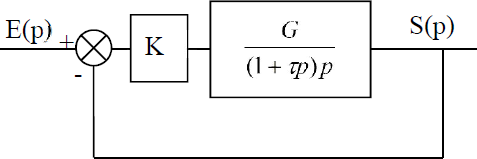
\includegraphics[width=\linewidth]{fig_02}
%\textit{}
\end{center}
Ils doivent répondre au cahier des charges suivant :
\begin{itemize}
\item précision de la position des pieds : écart statique inférieur à 5\%;
\item rapidité de l’asservissement : $t_{5\%} = \SI{0,15}{s}$;
\item stabilité : marge de phase de 45\degres, marge de gain de \SI{10}{dB} ;
\item sécurité du mouvement : aucun dépassement.
\end{itemize}

\subsection*{Modélisation du comportement du vérin}

Le comportement du vérin est régi par deux phénomènes : la dynamique de la tige du vérin et
les flux de débits dans les chambres.
\textbf{Données : }
\begin{itemize}
\item $S=12\times 10^{-4}\,\text{m}^2$, surface utile des pistons;
\item $ b = {10^9}\,\text{Pa}$ : module de compressibilité du fluide utilisé ;
\item $P_a = 150 \times 10^5\,\text{Pa}$ : pression d’alimentation de la servovalve ;
\item $K = \SI{e-7}{m^3s^{-1}V^{-1}Pa^{-.5}}$ : constante de débit de la servovalve ;
\item $\varphi = \SI{e-11}{m^3 Pa^{-1}}$ : facteur de fuite dans le vérin ;
\item $q(t )$ : débit entrant et sortant du vérin ;
\item $V_1$ et $V_2$ : volumes des deux chambres du vérin (hypothèse : $V_1 = V_2 = V = {6e-4}{m^3}$ ;
\item $p(t ) = p_1 -p_2$ : différence des pressions dans les chambres du vérin ;
\item $z (t )$ : déplacement de la tige par rapport à la position d’équilibre ;
\item $M = \SI{700}{kg}$ : masse équivalente pour chaque vérin, correspondant au quart de la masse
totale du robot ;
\item $k = \SI{e5}{Nm^{-1}}$ : raideur équivalente de la structure du robot ;
\item $\mu = \SI{100}{N.s.m^{-1}}$ : coefficient de frottement visqueux dans le vérin ;
\item $F_0 = \SI{3000}{N}$ : effort nominal sur le vérin ;
\item $Z_0 = \SI{50}{cm}$ : position nominale du vérin.
\end{itemize}
Le vérin est soumis à l’effort de forage, aux efforts de pression de l’huile et à une force de
frottement visqueux. Enfin, la rigidité de la structure du robot est modélisée par une raideur $k$ .

L’équation de résultante du PFD, projetée sur l’axe $\vect{z}$ du vérin, conduit à l’équation :

$$
M\dfrac{\dd^2 z(t)}{\dd t^2} = -\mu \dfrac{\dd z (t)}{\dd t} - k\left( z(t) - Z_0\right) +Sp(t)-F_{\text{forage}}(t).
$$

Le bilan de débit tient compte du déplacement de la tige du vérin évidemment, mais aussi du
débit de fuite entre les deux chambres du vérin et de la compressibilité de l’huile. Il conduit à
l’équation :
$$
q(t)=S \dfrac{\dd z (t)}{\dd t} +\varphi p(t) + \dfrac{V}{2b}  \dfrac{\dd p(t)}{\dd t}.
$$





\subparagraph{}\textit{Identifier, dans les équations du PFD et de bilan de débit, les termes correspondant :
\begin{itemize}
\item  l’inertie du robot;
\item à la raideur du robot;
\item  au frottement visqueux;
\item  à la pression dans la chambre;
\item  à la compressibilité de l’huile;
\item  au déplacement de la tige de vérin;
\item aux fuites entre les chambres.
\end{itemize}}
\ifprof
\begin{corrige}
Termes correspondant :
\begin{itemize}
\item  l’inertie du robot : $M\dfrac{\dd^2 z(t)}{\dd t^2}$;
\item à la raideur du robot : $ - k\left( z(t) - Z_0\right)$;
\item  au frottement visqueux : $ -\mu \dfrac{\dd z (t)}{\dd t}$;
\item  à la pression dans la chambre : $Sp(t)$;
\item  à la compressibilité de l’huile : $ \dfrac{V}{2b}  \dfrac{\dd p(t)}{\dd t}$;
\item  au déplacement de la tige de vérin : $ S \dfrac{\dd z (t)}{\dd t}$;
\item aux fuites entre les chambres : $\varphi p(t) $.
\end{itemize}
\end{corrige}
\else
\fi

\subparagraph{}\textit{En considérant une évolution au point de fonctionnement $P_0$, $F_0$ et $Z_0$, traduire l'équation d'équilibre du vérin.}
\ifprof
\begin{corrige}
On a : 
$M\dfrac{\dd^2 z(t)}{\dd t^2} = -\mu \dfrac{\dd z (t)}{\dd t} - k\left( z(t) - Z_0\right) +Sp(t)-F_{\text{forage}}(t)$. 
Au point de fonctionnement, on a donc $0 = SP_0-F_0$ et donc $SP_0 = F_0$.
\end{corrige}
\else
\fi



\subparagraph{}\textit{On considère maintenant une petite variation autour du point de fonctionnement. On pose alors $p(t ) = P_0 +\Delta p(t )$, $F_{\text{forage}(t )} = F_0 +\Delta F(t )$ et $z (t ) = Z_0 +\Delta z (t )$. Traduire l’équation de comportement du vérin en fonction des petites variations.}
\ifprof
\begin{corrige}
Au voisinage du point de fonctionnement, on a donc : $M\dfrac{\dd^2 \Delta z(t)}{\dd t^2} = -\mu \dfrac{\dd \Delta z (t)}{\dd t} - k\Delta z(t) +S\left( P_0 +\Delta p(t ) \right)-F_0 - \Delta F(t )$. De plus, à l'équilibre, $SP_0=F_0$. 
Dans le domaine de Laplace, on a alors $ \Delta Z(p)  \left( Mp^2 + \mu p +k\right) = S\Delta P(p) - \Delta F(p )$.
\end{corrige}
\else
\fi


\subparagraph{}\textit{En considérant une évolution au point de fonctionnement $P_0$, $Q_0$ et $Z_0$, traduire l'équation de bilan des débits.}
\ifprof
\begin{corrige}
On a $q(t)=S \dfrac{\dd z (t)}{\dd t} +\varphi p(t) + \dfrac{V}{2b}  \dfrac{\dd p(t)}{\dd t} $.
Au point de fonctionnement, on a donc $Q_0 = \varphi P_0$ .
\end{corrige}
\else
\fi




\subparagraph{}\textit{On considère maintenant une petite variation autour du point de fonctionnement. On pose alors $q(t ) = Q_0 +\Delta q(t )$. Traduire l’équation de comportement du vérin en fonction des petites variations.}
\ifprof
\begin{corrige}
Au voisinage du point de fonctionnement, on a donc  


$ Q_0 +\Delta q(t )=S \dfrac{\dd \left(Z_0 +\Delta z (t )\right)}{\dd t} +\varphi \left( P_0 +\Delta p(t ) \right) + \dfrac{V}{2b}  \dfrac{\dd \left(P_0 +\Delta p(t )\right)}{\dd t}$

$ \Leftrightarrow Q_0 +\Delta q(t )=S \dfrac{\dd \Delta z (t )}{\dd t} +\varphi \left( P_0 +\Delta p(t ) \right) + \dfrac{V}{2b}  \dfrac{\dd \Delta p(t )}{\dd t}$

$ \Leftrightarrow \Delta q(t )=S \dfrac{\dd \Delta z (t )}{\dd t} +\varphi  \Delta p(t ) + \dfrac{V}{2b}  \dfrac{\dd \Delta p(t )}{\dd t}$ (en utilisant la question précédente).

Dans le domaine de Laplace, on a donc $  \Delta Q(p)=S p\Delta Z(p ) +\varphi  \Delta P(p) + \dfrac{V}{2b}  p \Delta P(p)$ soit 
$  \Delta Q(p)=S p\Delta Z(p ) + \Delta P(p)\left(\varphi  + \dfrac{V}{2b}  p\right)$


\end{corrige}
\else
\fi

%
%
%
%On a aussi $q(t)=S \dfrac{\dd z (t)}{\dd t} +\varphi p(t) + \dfrac{V}{2b}  \dfrac{\dd p(t)}{\dd t}$. 
%
%
%
%
%
%
% et en
%posant $p(t ) = P_0 +\Delta p(t )$, $F_{\text{forage}(t )} = F_0 +\Delta F(t )$ et $z (t ) = Z_0 +\Delta z (t )$, traduire l’équation d’équilibre du vérin au point de fonctionnement, puis traduire l’équation de comportement
%du vérin en fonction des petites variations.}
%\ifprof
%\begin{corrige}
%On a : $
%M\dfrac{\dd^2 z(t)}{\dd t^2} = -\mu \dfrac{\dd z (t)}{\dd t} - k\left( z(t) - Z_0\right) +Sp(t)-F_{\text{forage}}(t)
%$. 
%Au voisinage du point de fonctionnement, on a donc : $
%M\dfrac{\dd^2 \Delta z(t)}{\dd t^2} = -\mu \dfrac{\dd \Delta z (t)}{\dd t} - k\Delta z(t) +S\left( P_0 +\Delta p(t ) \right)-F_0 - \Delta F(t )$. De plus, à l'équilibre, $SP_0=F_0$. 
%
%Dans le domaine de Laplace, on a alors $ \Delta Z(p)  \left( Mp^2 + \mu p +k\right) = S+\Delta p(p) - \Delta F(p )
%$.
%
%
%
%On a aussi $q(t)=S \dfrac{\dd z (t)}{\dd t} +\varphi p(t) + \dfrac{V}{2b}  \dfrac{\dd p(t)}{\dd t}$. 
%\end{corrige}
%\else
%\fi

\subparagraph{}\textit{À partir des équations obtenues, compléter le le schéma-blocs traduisant son comportement.}
\ifprof
\begin{corrige}
\end{corrige}
\else
\fi

\begin{center}
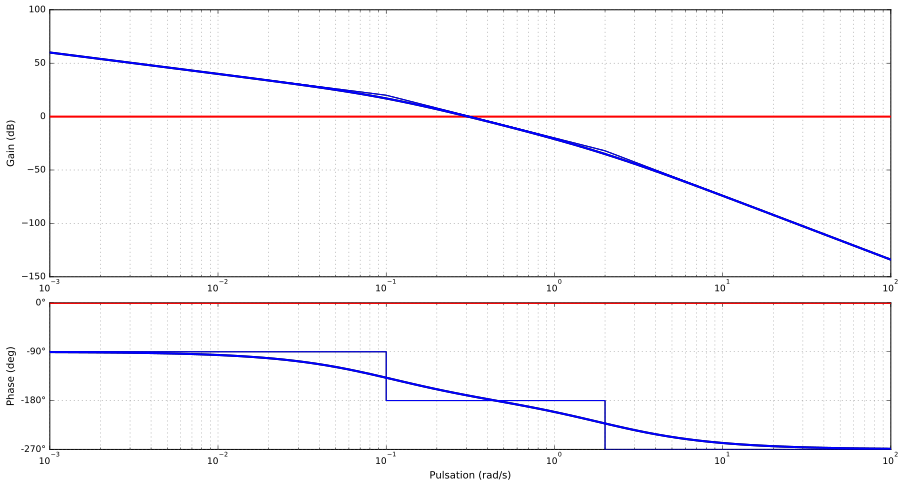
\includegraphics[width=\linewidth]{fig_03}
%\textit{}
\end{center}



\subsection*{Modélisation du comportement de la servovalve}
La servovalve permet de fournir le débit $q(t )$ au vérin à partir d’une tension de commande
$u(t )$ appliquée en entrée : la tension $u(t )$ est imposée aux bornes d’une bobine qui déplace le
tiroir, permettant de distribuer l’énergie hydraulique. Elle est alimentée en entrée à une pression
constante $p_a$ et la sortie est à la pression relative nulle.
Le débit dépend directement du déplacement du tiroir et donc de la tension $u(t )$, mais également
de la différence de pression dans les chambres du vérin, par la relation non linéaire :
$q(t ) = Ku(t) \sqrt{p_a-p(t)}$.
 
Afin d’implanter le comportement de la servovalve dans une modélisation linéaire, il est nécessaire
de procéder à une linéarisation au voisinage d’un point de fonctionnement.

\subparagraph{}\textit{Déterminer la relation liant $Q_0$, $U_0$ et $P_0$ au point de fonctionnement (en considérant qu'en ce point les variations de tension, pressions et débit sont nulles).  Linéariser l’équation de comportement de la servovalve au voisinage du point de fonctionnement. On posera
$p(t ) = P_0 +\Delta p(t )$, $q(t ) =Q_0 +\Delta q(t )$ et $u(t ) =U_0 +\Delta u(t )$.}
\ifprof
\begin{corrige}
Au point de fonctionnement,  $Q_0 = K U_0 \sqrt{p_a- P_0}$.

Par ailleurs, on a  

$Q_0 +\Delta q(t ) = K\left( U_0 +\Delta u(t ) \right) \sqrt{p_a- P_0 - \Delta p(t )}$

$\Leftrightarrow K U_0 \sqrt{p_a- P_0}+\Delta q(t ) = K\left( U_0 +\Delta u(t ) \right) \sqrt{p_a- P_0 - \Delta p(t )}$

$\Leftrightarrow K U_0 \sqrt{p_a- P_0}+\Delta q(t ) = K\left( U_0 +\Delta u(t ) \right) \sqrt{\left(p_a- P_0\right)\left( 1- \dfrac{\Delta p(t )}{p_a- P_0}\right)}$

et $\sqrt{ 1- \dfrac{\Delta p(t )}{p_a- P_0}}\simeq 1 - \dfrac{1}{2} \dfrac{\Delta p(t )}{p_a- P_0} $.

Soit $K U_0 \sqrt{p_a- P_0}+\Delta q(t ) = K\left( U_0 +\Delta u(t ) \right) \sqrt{p_a- P_0} \left( 1 - \dfrac{1}{2} \dfrac{\Delta p(t )}{p_a- P_0} \right)$

$\Leftrightarrow K U_0 \sqrt{p_a- P_0}+\Delta q(t ) = K\left( U_0 +\Delta u(t ) \right) \sqrt{p_a- P_0} - \dfrac{K\left( U_0 +\Delta u(t ) \right) \sqrt{p_a- P_0}}{2} \dfrac{\Delta p(t )}{p_a- P_0} $


$\Leftrightarrow K U_0 \sqrt{p_a- P_0}+\Delta q(t ) = K\left( U_0 +\Delta u(t ) \right) \sqrt{p_a- P_0} 
- \dfrac{K U_0  \sqrt{p_a- P_0}}{2} \dfrac{\Delta p(t )}{p_a- P_0}
- \underbrace{\dfrac{K\Delta u(t ) \sqrt{p_a- P_0}}{2} \dfrac{\Delta p(t )}{p_a- P_0}}_{\text{on néglige}} $


$\Leftrightarrow \Delta q(t ) = K\Delta u(t )  \sqrt{p_a- P_0} 
- \dfrac{K U_0 }{2} \dfrac{\Delta p(t )}{ \sqrt{p_a- P_0}}
 $

\end{corrige}
\else
\fi

\subparagraph{}\textit{Compléter le schéma-blocs précédent pour modéliser l’ensemble servovalve et vérin, admettant
en entrée la tension $\Delta U(p)$ et la force $\Delta F(p)$, et en sortie la position $\Delta Z(p)$.}
\ifprof
\begin{corrige}
\end{corrige}
\else
\fi

\subsection*{Asservissement de position}

Le vérin hydraulique est placé dans une boucle d’asservissement de position constituée de :
\begin{itemize}
\item la servovalve, qui fournit le débit $q(t )$ au vérin à partir d’un signal de commande $u(t)$ ;
\item un capteur de position de fonction de transfert $k_c$ , qui fournit une tension $\text{Im}(z (t ))$ image
de la position réelle $z (t )$;
\item un correcteur $C(p)$ qui élabore la commande $u(t )$ de la servovalve à partir de l’écart obtenu
entre $\text{Im}(z c (t ))$, image de la consigne de position, et $\text{Im}(z (t ))$.
$\text{Im}(zc (t ))$ est obtenue grâce à un adaptateur $K_a$ situé à l’extérieur de la boucle d’asservissement.
\end{itemize}


\subparagraph{}\textit{Compléter le schéma-bloc de l’asservissement ébauché.}
\ifprof
\begin{corrige}
\end{corrige}
\else
\fi

\subparagraph{}\textit{Préciser l’expression de l’adaptateur $K_a$ pour que l’écart soit nul lorsque la réponse est égale
à la consigne.}
\ifprof
\begin{corrige}
\end{corrige}
\else
\fi


Le schéma-blocs obtenu est mis sous la forme du schéma  où $A$, $B$, $C$, $D$, $E$, et $G$
sont utilisés pour simplifier les calculs.

\subparagraph{}\textit{À partir de modifications simples du schéma-bloc, déterminer la $\text{FTBO}$ de l’asservissement
en position du vérin selon les fonctions de transfert de la figure suivante. Exprimer la $\text{FTBF}$ de
l’asservissement en position du vérin en fonction de la $\text{FTBO}$.}
\ifprof
\begin{corrige}
\end{corrige}
\else
\fi


\begin{center}
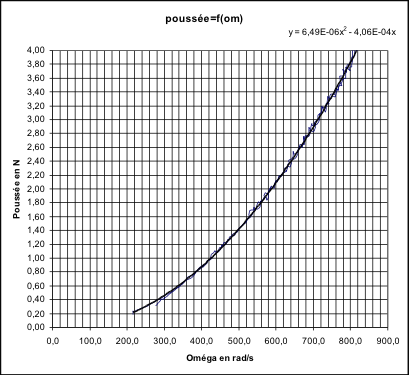
\includegraphics[width=\linewidth]{fig_04}
%\textit{}
\end{center}

\subsection*{Validation des performances pour une correction unitaire $C(p) = 1$}

Le calcul sur Scilab a permis d’obtenir l’expression numérique de la fonction de transfert en
boucle fermée, $\text{FTBF}(p) = \dfrac{0,975}{1+3,38\times 10^{-2}p+1,78\times 10^{-4}p^2+4,8\times 10^{-6}p^3}$, ainsi que les valeurs numériques des pôles : $p_{12}=-3,19 \pm 82,5 j$ et $p_3 = -30,4$ (en rad/s).

\subparagraph{}\textit{Le système est-il stable ? Est-il précis ?}
\ifprof
\begin{corrige}
\end{corrige}
\else
\fi


\subparagraph{}\textit{À partir des pôles de la FTBF, déterminer le(s) pôle(s) dominant(s) et en déduire une valeur
approchée du temps de réponse à 5\%.}
\ifprof
\begin{corrige}
\end{corrige}
\else
\fi


\subparagraph{}\textit{À partir des pôles de la FTBF, déterminer si le système est susceptible d’avoir des dépassements.}
\ifprof
\begin{corrige}
\end{corrige}
\else
\fi

Le calcul sur Scilab a permis d’obtenir l’expression numérique de la fonction de transfert en boucle
ouverte, $\text{FTBO}(p) = \dfrac{38,6}{1+1,33\times 10^{-2}p+7,03\times 10^{-3}p^2+1,9\times 10^{-4}p^3}$, ainsi que les valeurs numériques des pôles : $p_{12}=-18 \pm 81,6 j$ et $p_3 = -0,75$ (rad/s)

\subparagraph{}\textit{Déterminer la valeur de la pulsation propre et le facteur d’amortissement du deuxième ordre,
puis tracer les diagrammes de Bode asymptotiques de la FTBO et l’allure des diagrammes
réels. Déterminer les marges de gain et de phase du système corrigé par un gain unitaire.}
\ifprof
\begin{corrige}
\end{corrige}
\else
\fi



\subsection*{Optimisation du comportement : réduction des oscillations}
La solution retenue pour atténuer la résonance est l’utilisation d’un filtre dit « réjecteur », de
fonction de transfert :
$C(p)=\dfrac{1+\dfrac{2\xi_1}{\omega_0}p+\dfrac{p^2}{\omega_0^2}}{1+\dfrac{2\xi_2}{\omega_0}p+\dfrac{p^2}{\omega_0^2}}$ avec $\xi_1 < \xi_2 < \dfrac{\sqrt{2}}{2}$.

\subparagraph{}\textit{Tracer l’allure du diagramme de Bode en gain, asymptotique et réel de ce correcteur et
expliquer son mode de fonctionnement.}
\ifprof
\begin{corrige}
\end{corrige}
\else
\fi

On choisit de prendre $\omega_0$ égal à la pulsation de résonance de la boucle ouverte et $\xi_2 = 0,7$.


\subparagraph{}\textit{Proposer une valeur pour le paramètre $\xi_1$. Le cahier des charges sera-t-il validé (aucun
calcul n’est attendu pour cette question, hormis des applications numériques simples).}
\ifprof
\begin{corrige}
\end{corrige}
\else
\fi




\subsection*{Éléments de correction}
\begin{enumerate}
\item ...
\item $\left(Mp^2+\mu p + k \right)\Delta Z(p) = S\Delta p (p)-\Delta F(p)$ et $\Delta Q(p)=S p \Delta Z(p) + \left( \varphi + \dfrac{V}{2b} p \right) \Delta P(p)$.
\item ...
\item $\Delta q = K\Delta U\sqrt{p_a - P_0} - \dfrac{KU_0}{2\sqrt{p_a - P_0}}\Delta p + \text{termes néglig.}$.
\item ...
\item ...
\item $K_a = k_c$.
\item $\text{FTBO}(p)=\dfrac{ABC(p)GE}{1+GDB+GE}$ et $\text{FTBF}(p)=\dfrac{\text{FTBO}(p)}{1+\text{FTBO}(p)}$.
\item ...
\item ...
\item ...
\item $\omega_0=\SI{83,6}{rad.s^{-1}}$ et $\xi=0,21$, $\omega_3 = \SI{0,75}{rad.s^{-1}}$.
\item ...
\item ...
\end{enumerate}


\ifprof
\else
\end{multicols}
\fi





%\subparagraph{}\textit{}
%\ifprof
%\begin{corrige}
%\end{corrige}
%\else
%\fi
%
%\begin{center}
%\includegraphics[width=\linewidth]{}
%%\textit{}
%\end{center}
%\begin{center}
%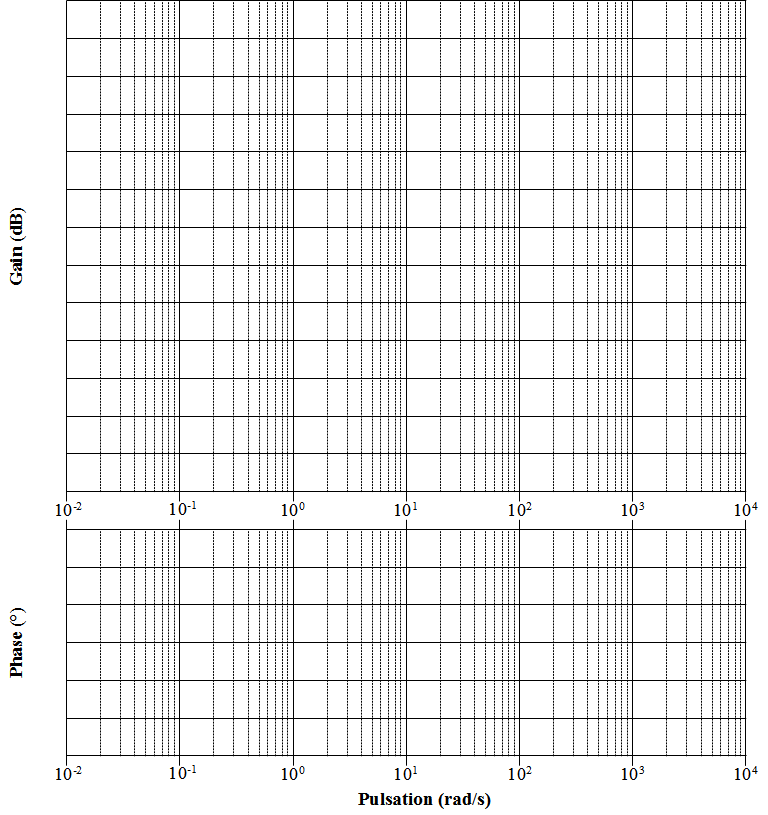
\includegraphics[width=\linewidth]{img_04}
%%\textit{}
%\end{center}

